\documentclass[ignorenonframetext]{beamer}
\usetheme{PaloAlto}
\usecolortheme{seagull}
\usefonttheme{structurebold}

\pgfdeclareimage[height=.75cm]{university-logo}{images/TAM_Logo1}
\logo{\pgfuseimage{university-logo}}

	\subject{Time Series Analysis}
	% This is only inserted into the PDF information catalog. Can be left
	% out. 
\usepackage{group4}
\usepackage{verbatimbox}

\begin{document}
\begin{frame}
	\titlepage
\end{frame}


	\section*{Outline}
	\begin{frame}{Outline}
		\tableofcontents
	\end{frame}
	
\section{Description of data}

 %-------------------------------------------------------------------------------------------------- 
  	\begin{frame}{Timplot of National Unemployment}
		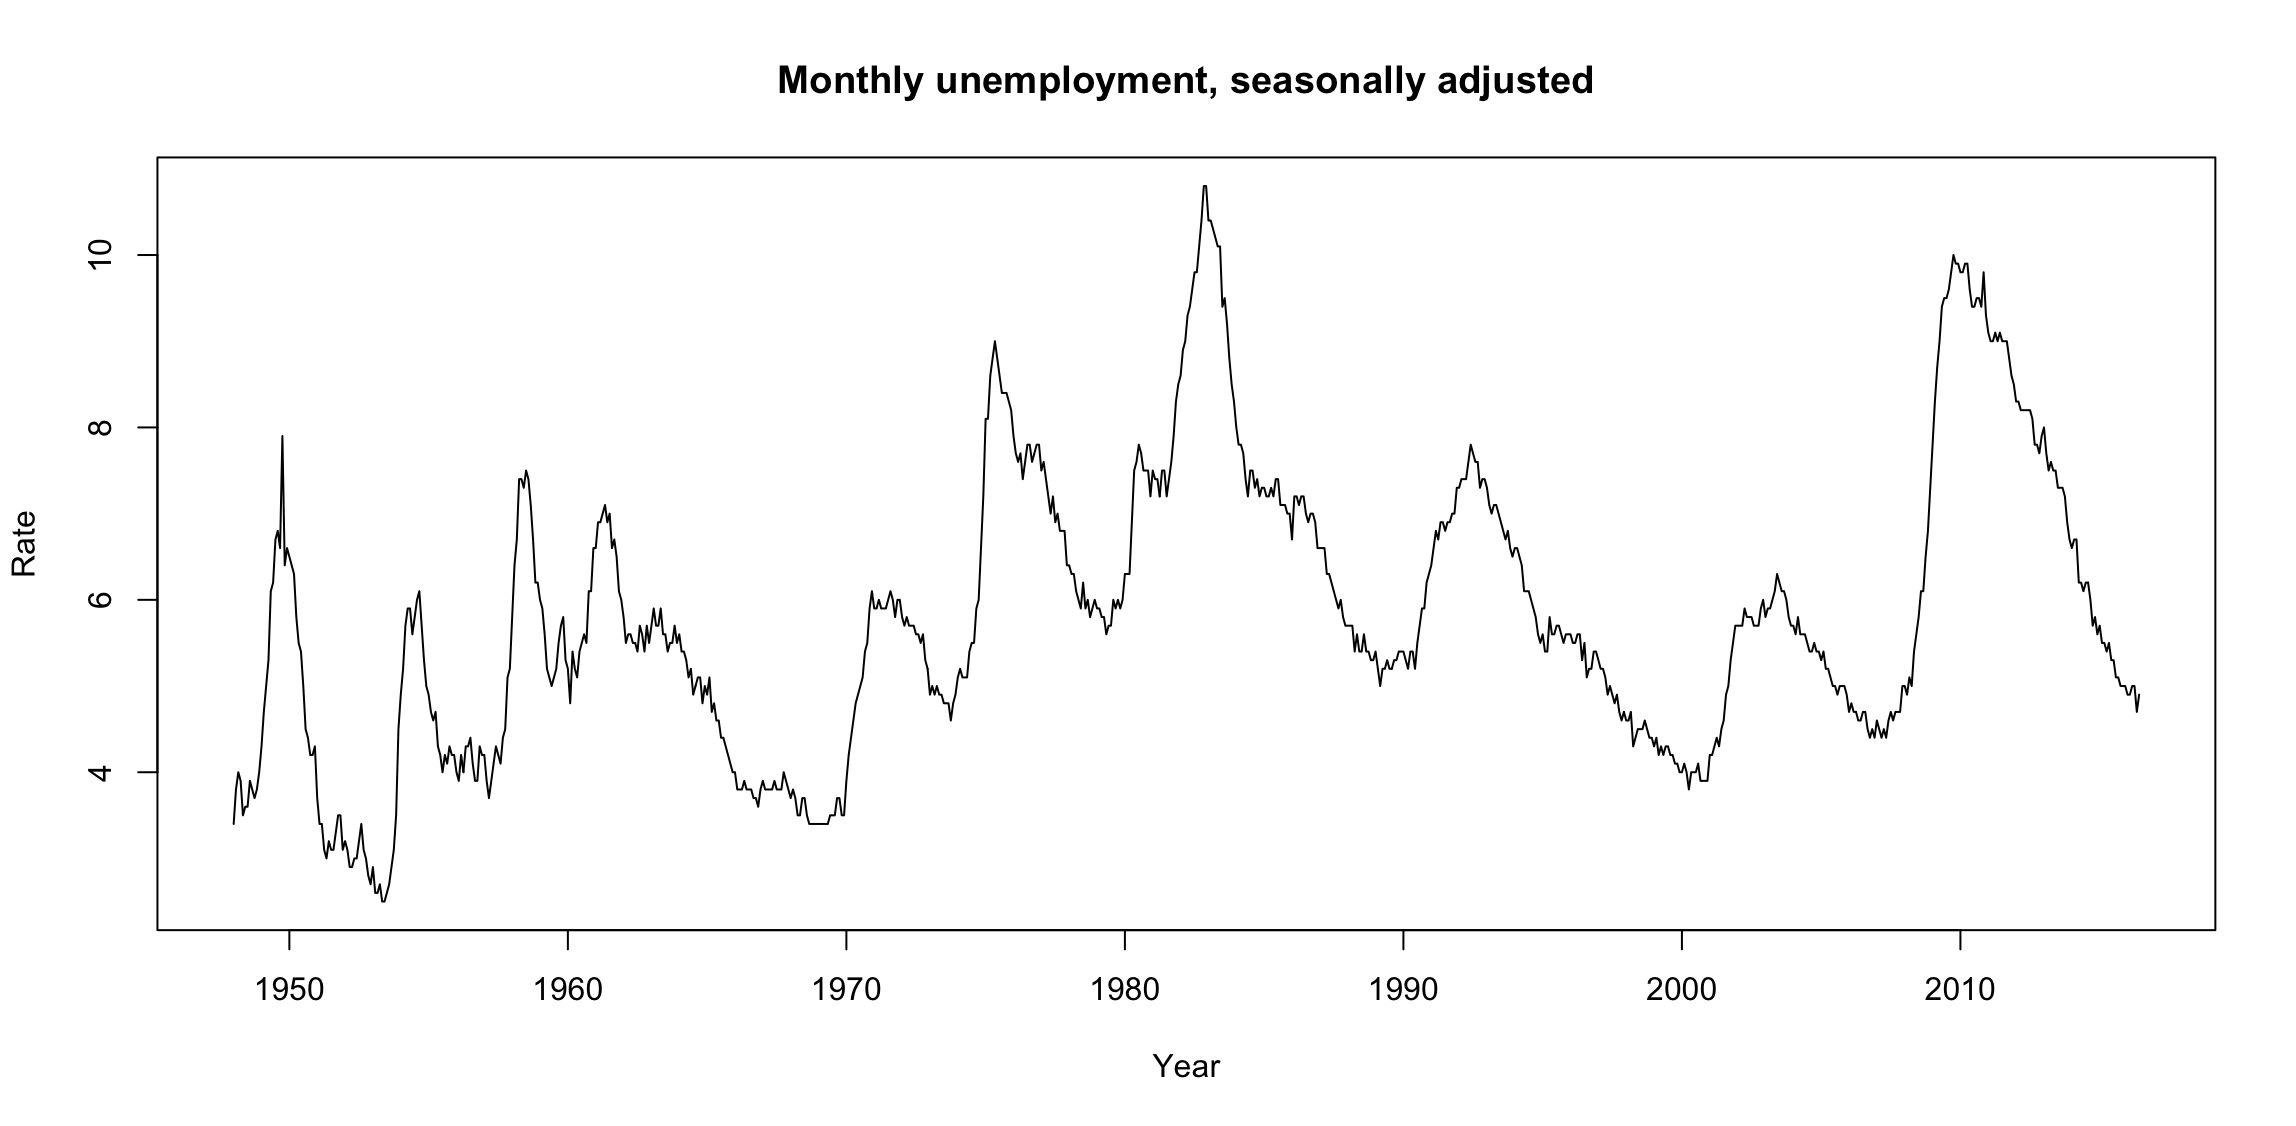
\includegraphics[width=\textwidth]{images/unemployment_total_sa}
  	\end{frame}
 %-------------------------------------------------------------------------------------------------- 
 
 %--------------------------------------------------------------------------------------------------  	
  	\begin{frame}{Smoothed unemployment for the study time period}
		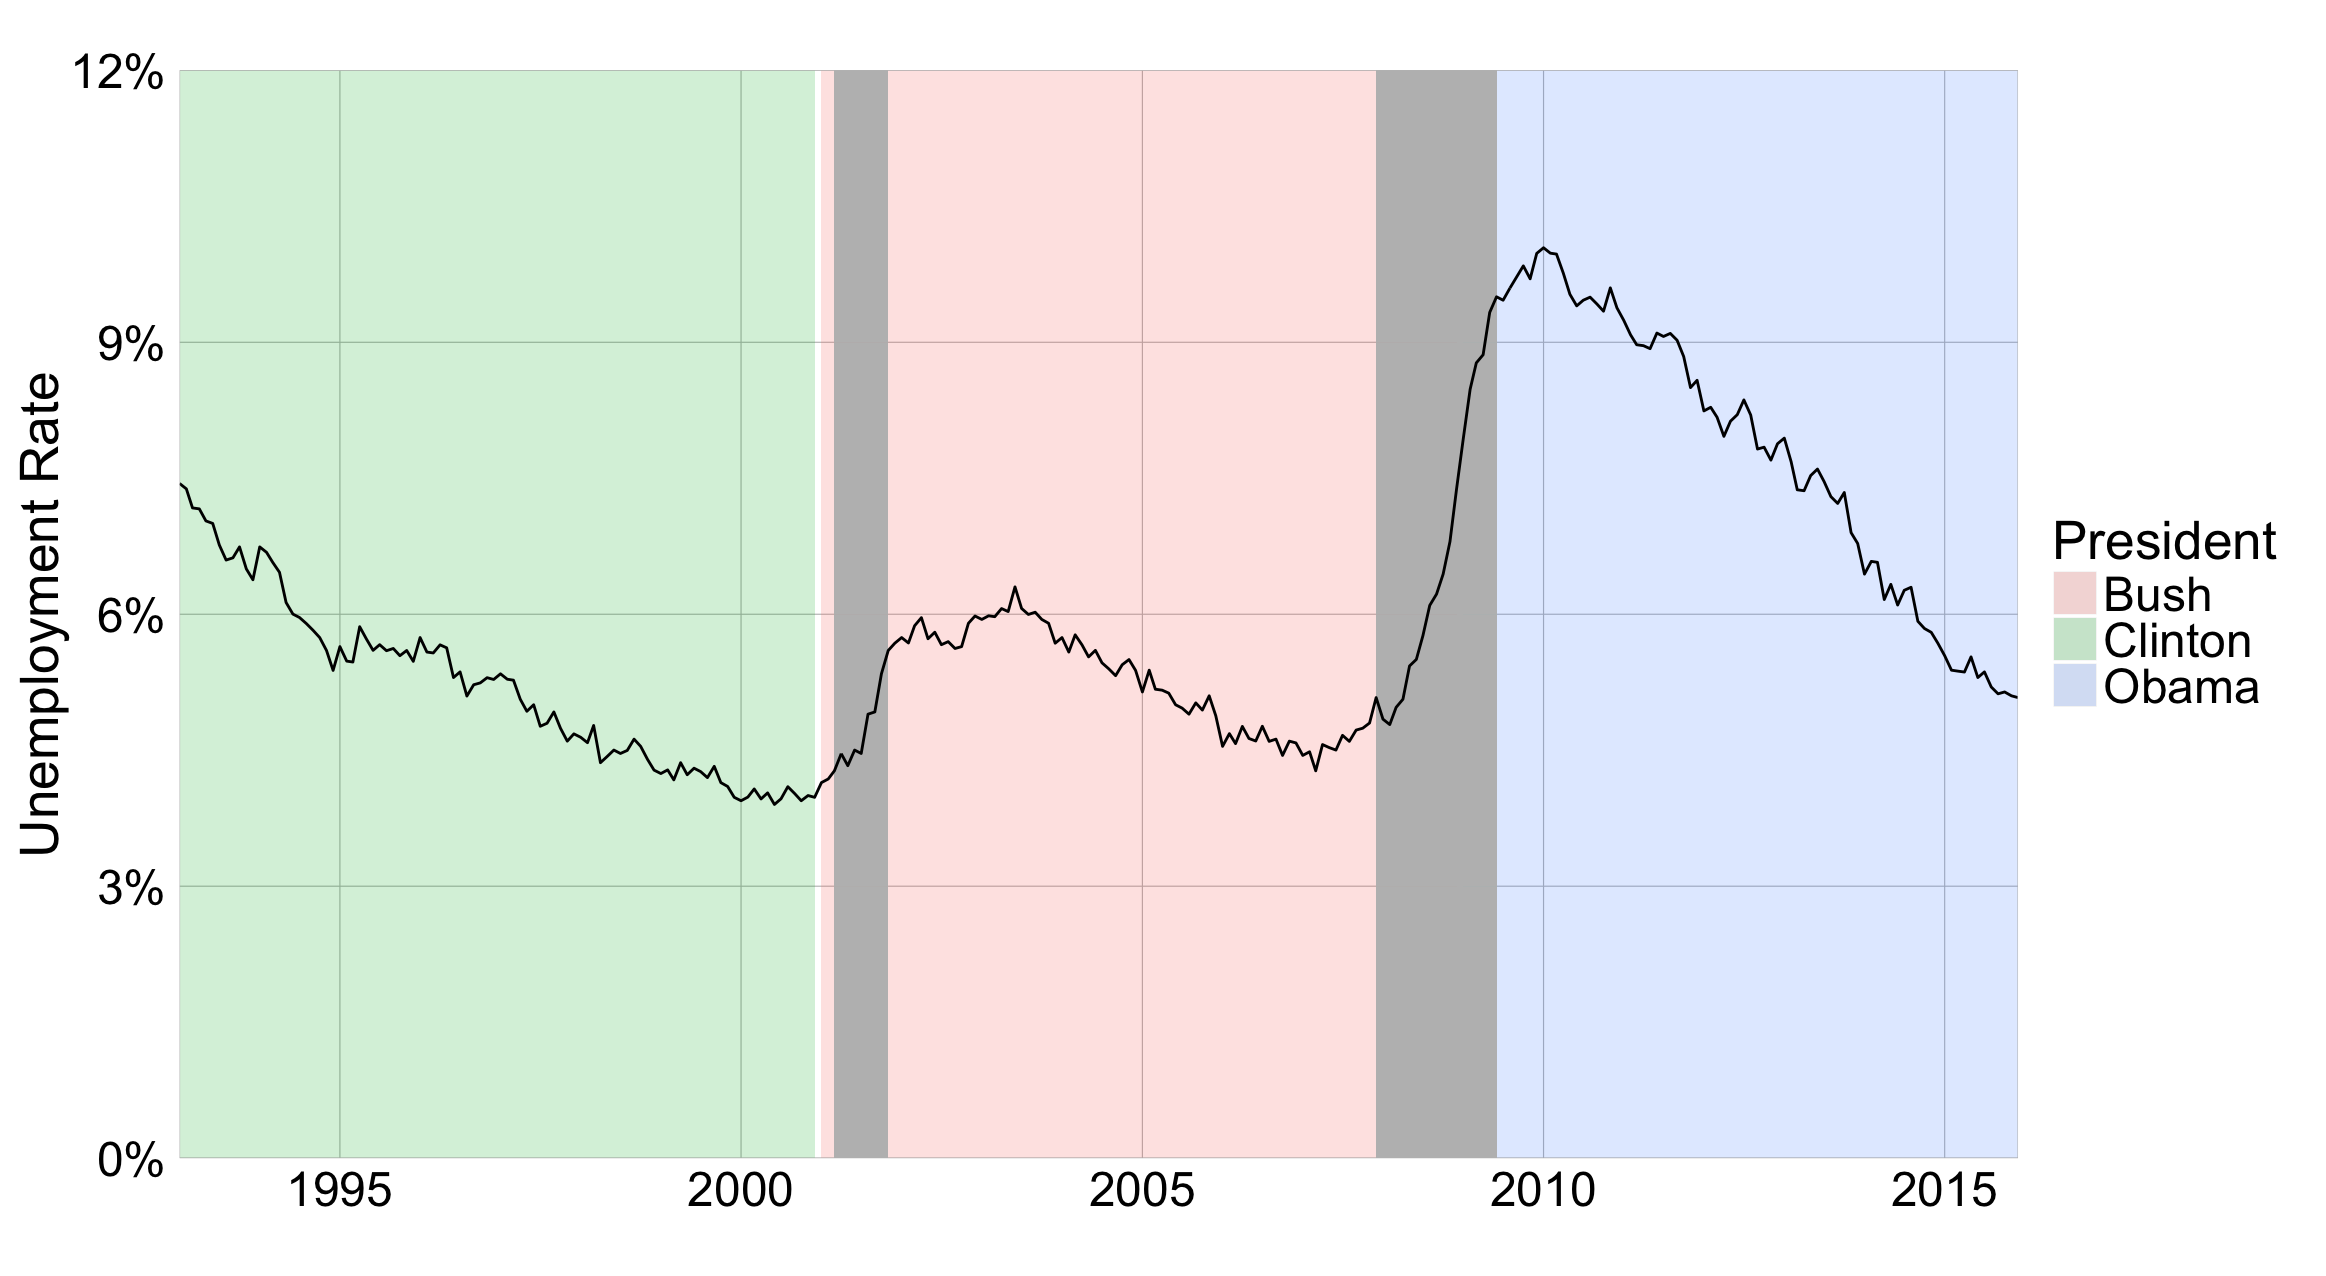
\includegraphics[width=\linewidth]{images/presunemp}
  	\end{frame}
%--------------------------------------------------------------------------------------------------  	

%--------------------------------------------------------------------------------------------------  	
\begin{frame}{Scatterplot matrix of unemployment and potential predictors}
		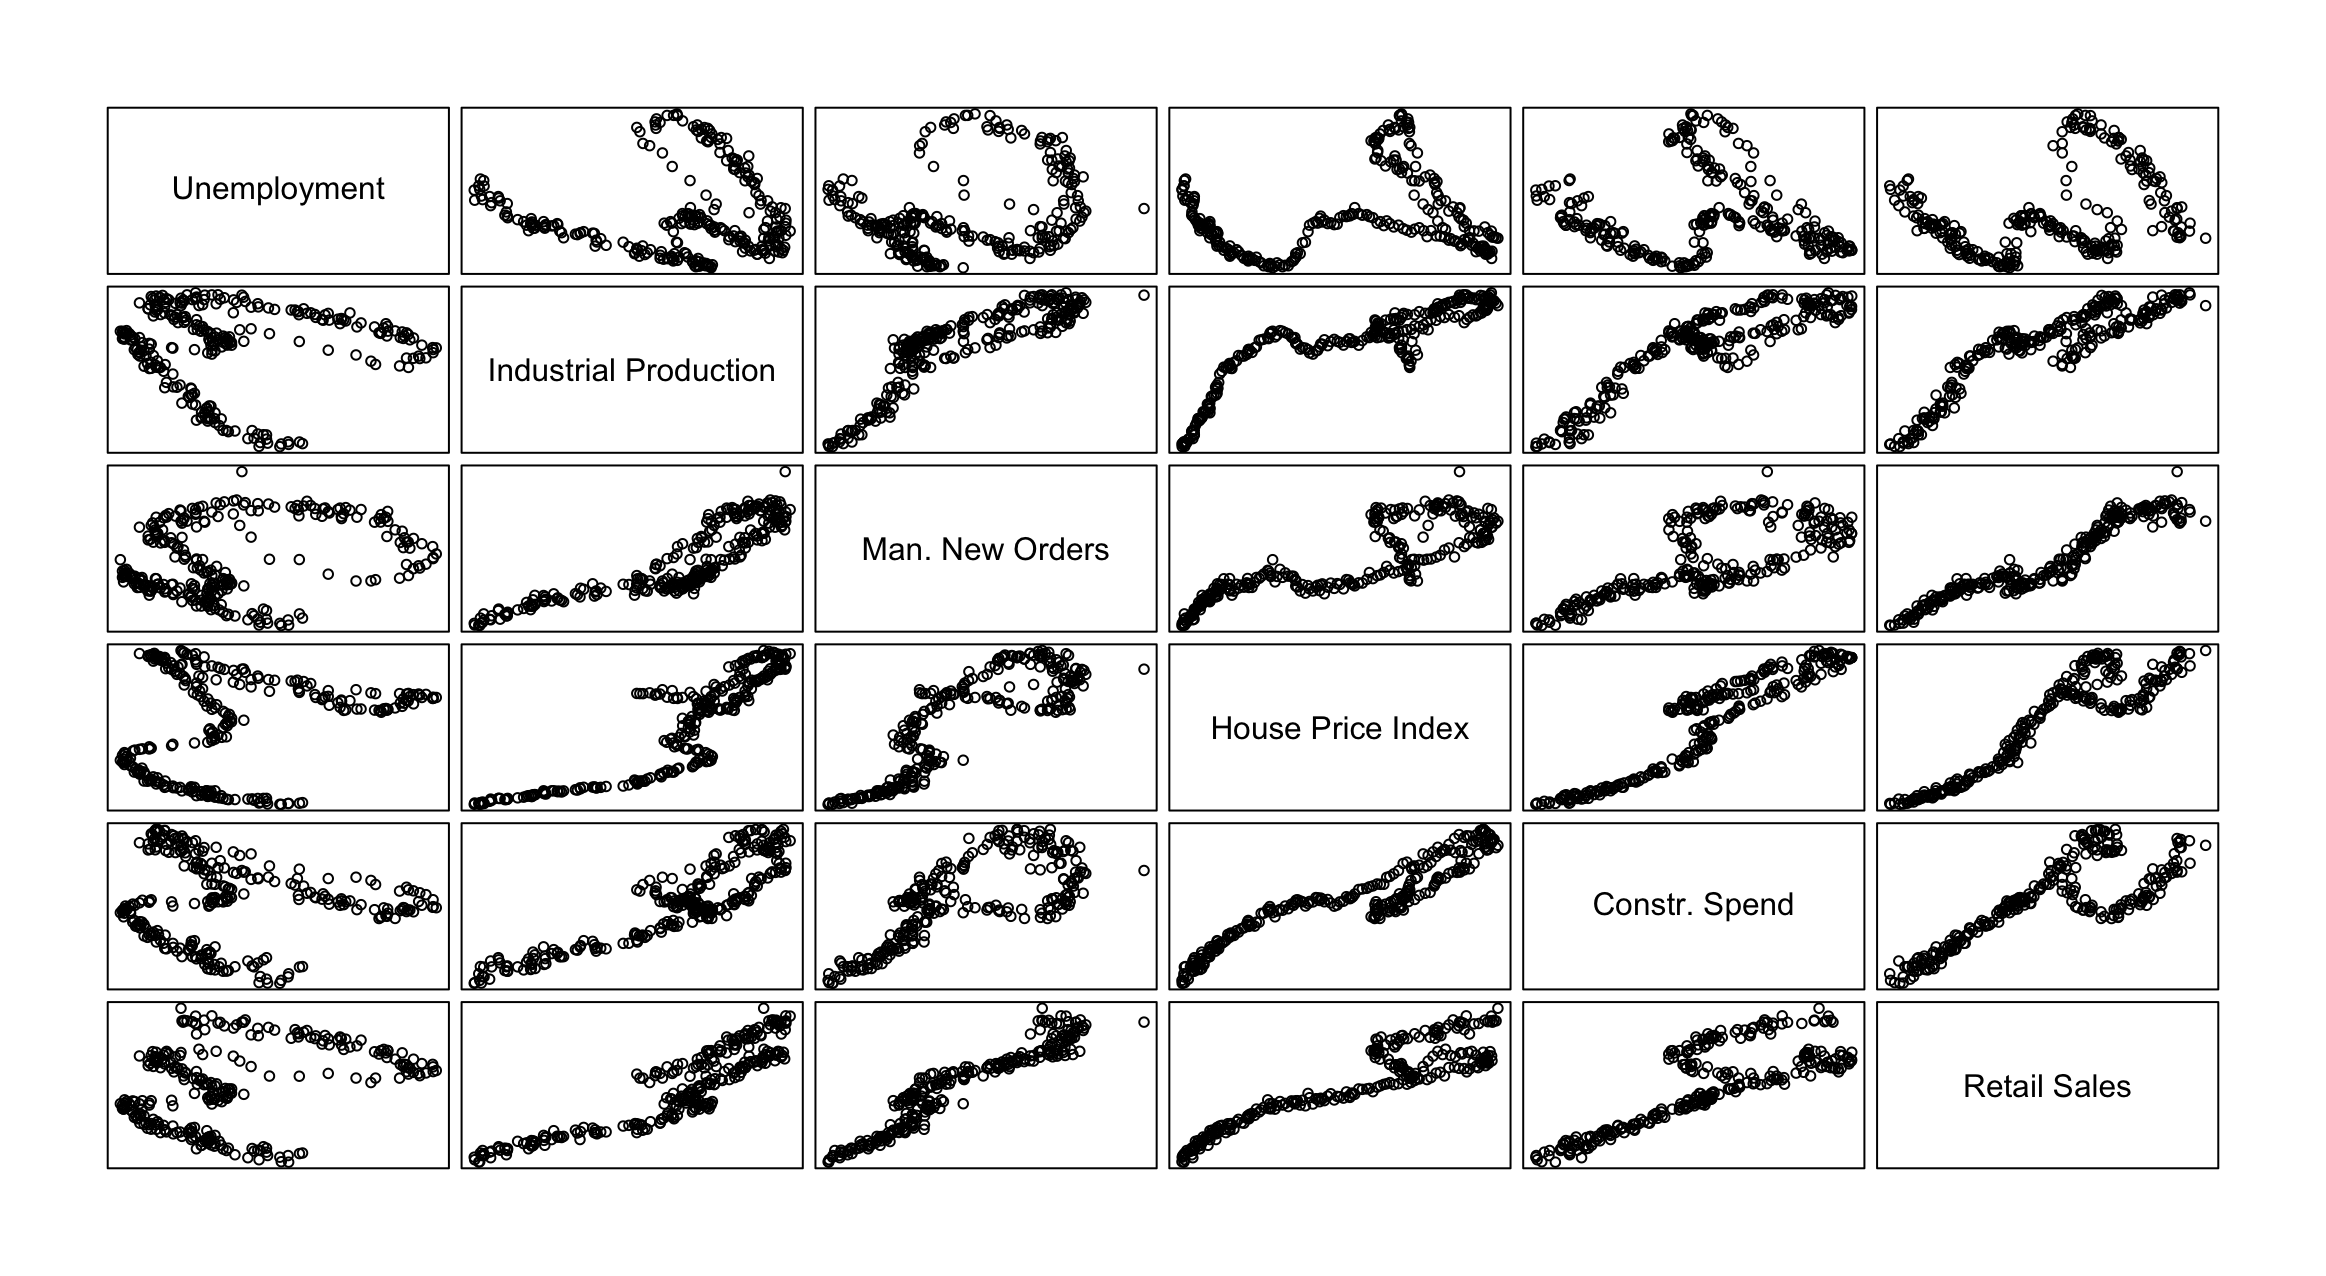
\includegraphics[width=\linewidth]{images/pred_scatt}
\end{frame}
%--------------------------------------------------------------------------------------------------  	


%-------------------------------------------------------------------------------------------------- 
    \begin{frame}[fragile]{Decomposition of Data}
\begin{verbnobox}[\tiny]
----------------------------------------------------------------------------------
decom.unem = decompose(ts(data = econ$unem_rate, 
             start = c(1993,1), frequency = 12), type = "additive")
decom.ind = decompose(ts(data = econ$industrial_production_index, 
                         start = c(1993,1), frequency = 12), type = "additive")
decom.mno = decompose(ts(data = econ$manufacturers_new_orders, 
                         start = c(1993,1), frequency = 12), type = "additive")
decom.hpi = decompose(ts(data = econ$purchase_house_price_index, 
                         start = c(1993,1), frequency = 12), type = "additive")
decom.con = decompose(ts(data = econ$construction_spending, 
                         start = c(1993,1), frequency = 12), type = "additive")
decom.rts = decompose(ts(data = econ$retail_sales, 
                         start = c(1993,1), frequency = 12), type = "additive")
                         
----------------------------------------------------------------------------------

## Seasonally Adjust 2016 unemployment
unem.16 = unem.16 - decom.unem$seasonal[1:5]

----------------------------------------------------------------------------------
## Add seasonally adjusted rate
econ.sa = data.frame(
  row.names = row.names(econ),
  unem_rate_sa = econ$unem_rate - decom.unem$sea,
  industrial_production_sa = econ$industrial_production_index - decom.ind$sea,
  manufacturers_new_orders_sa = econ$manufacturers_new_orders - decom.mno$sea,
  house_price_sa = econ$purchase_house_price_index - decom.hpi$sea,
  construction_spend_sa = econ$construction_spending - decom.con$sea,
  retail_sales_sa = econ$retail_sales - decom.rts$sea,
  recession_ind = econ$recession_ind
)
----------------------------------------------------------------------------------
\end{verbnobox}
\end{frame}
 %--------------------------------------------------------------------------------------------------
 
 %--------------------------------------------------------------------------------------------------  	
\begin{frame}{Autocorrelation of unemployment data}
		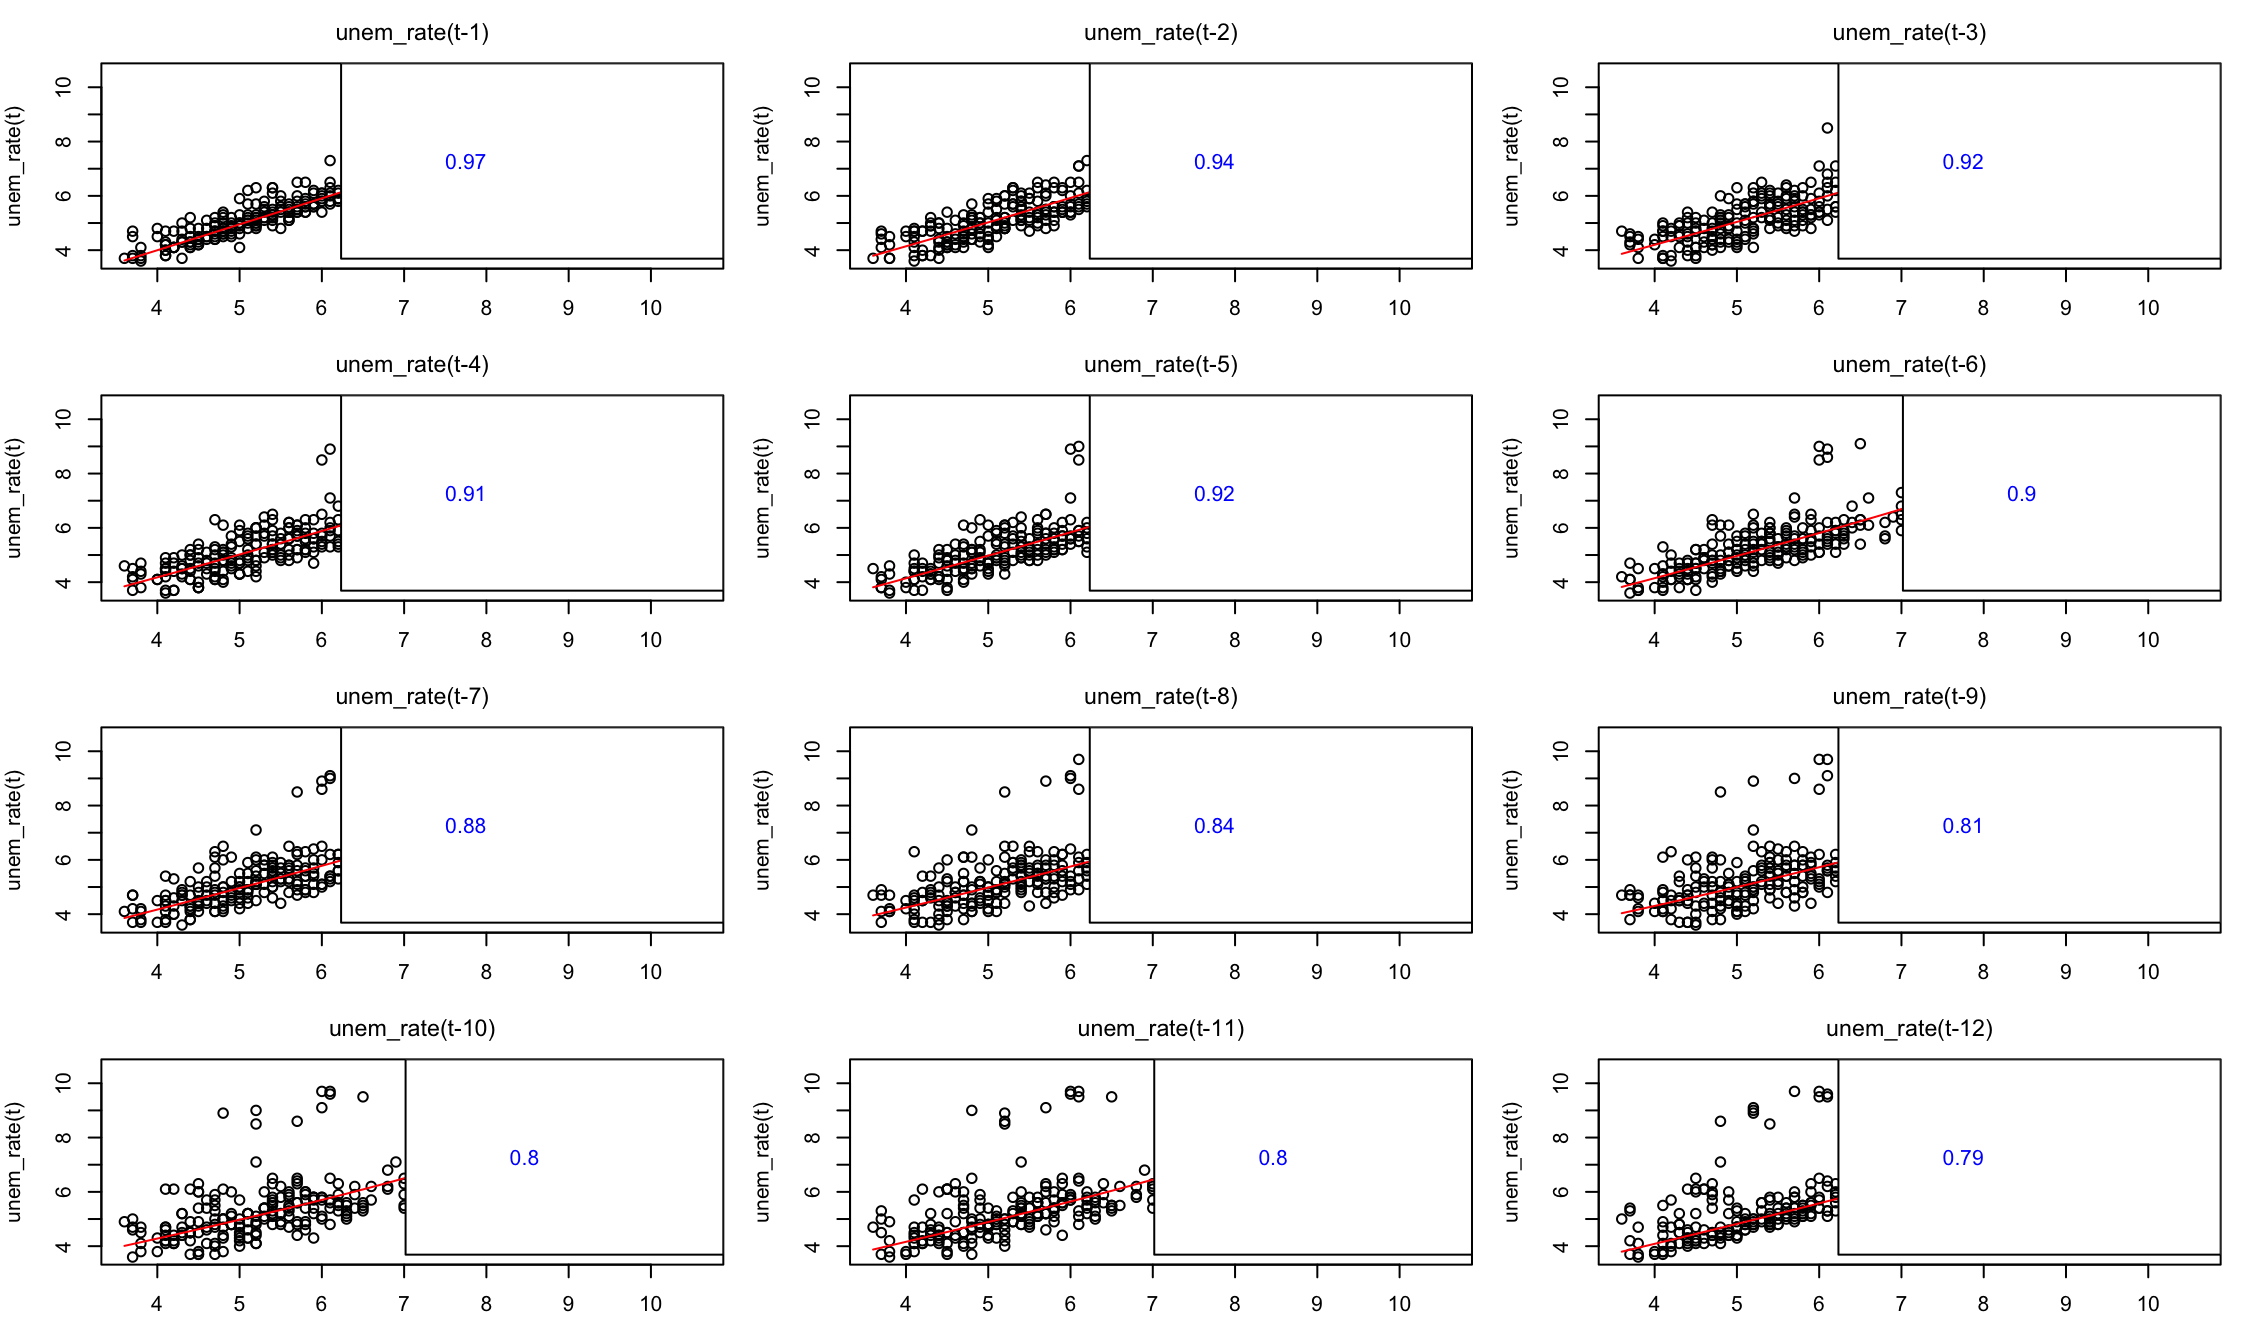
\includegraphics[width=\linewidth]{images/laggedunemployment}
\end{frame}
%--------------------------------------------------------------------------------------------------  	
 

 %-------------------------------------------------------------------------------------------------- 
  	\begin{frame}{Timeplots with and without differencing}
		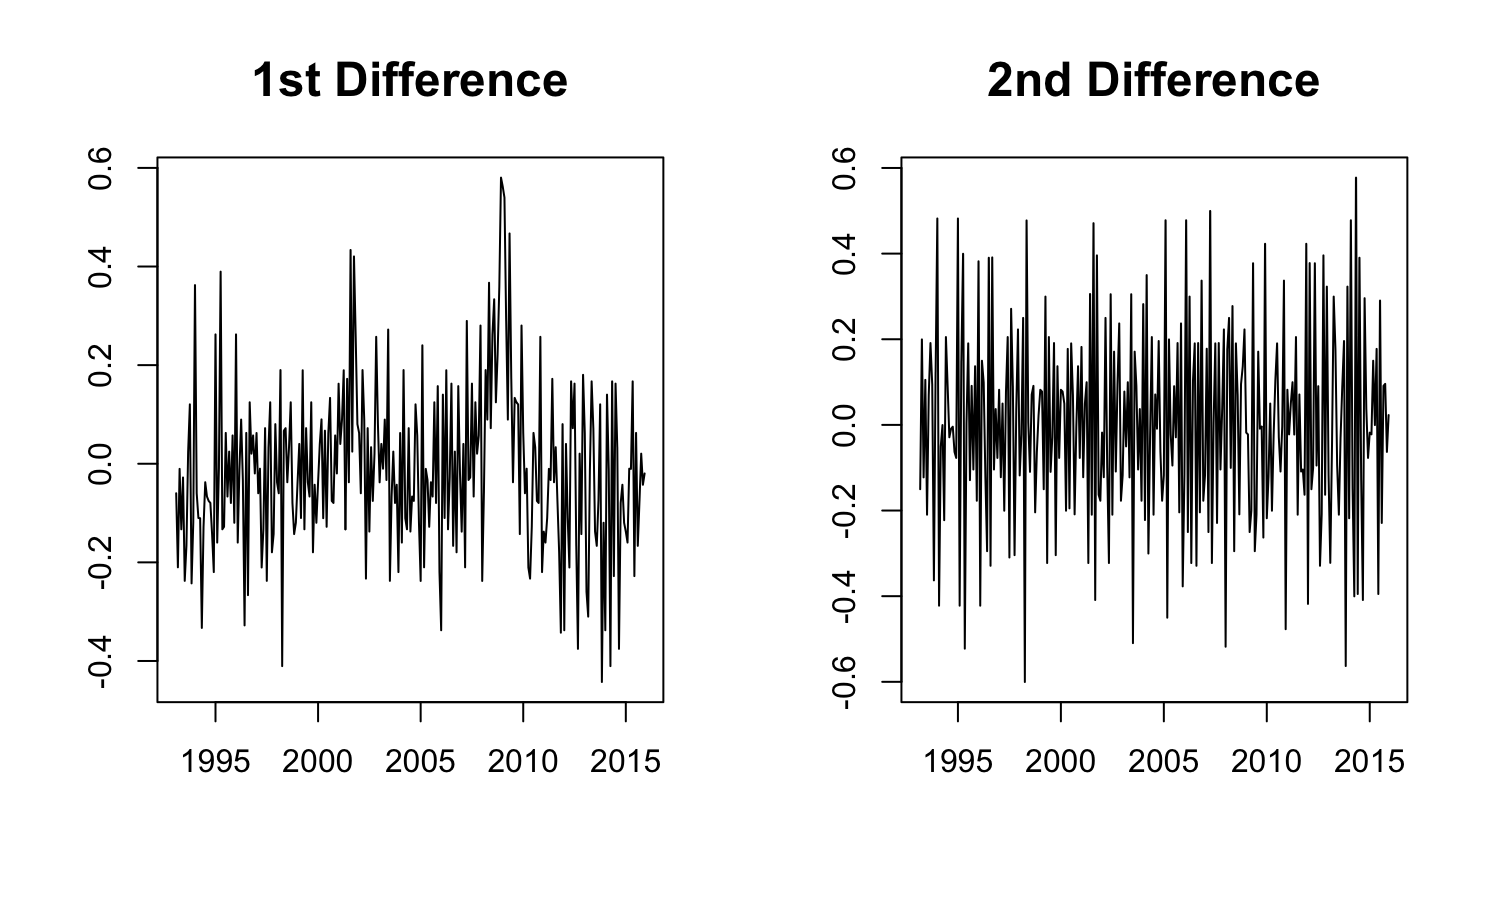
\includegraphics[width=\linewidth]{images/seasonalunem}
  	\end{frame}
 %--------------------------------------------------------------------------------------------------
 
 %-------------------------------------------------------------------------------------------------- 
  	\begin{frame}{ADF Test Results for unemployment}
		 \begin{table}[htb]
		 \centering
		 \begin{tabular}{lllll}
		 \hline
		 \textbf{Model} & \textbf{Statistic} & \textbf{Lag order} & \textbf{p-value}\\ \hline
		  1\(^{st}\) difference &  -9.3595 & 6 &\( < 0.01\)\\
		  2\(^{nd}\) difference &  -9.3595 & 6 & \( < 0.01\)\\			  
		  3\(^{rd}\) difference &  -13.02 & 6 & \( < 0.01\)\\		 \hline
		 \end{tabular}
		 \end{table}
  	\end{frame}
 %-------------------------------------------------------------------------------------------------- 
 
  %-------------------------------------------------------------------------------------------------- 
  	\begin{frame}{Timeplots of differenced predictors}
		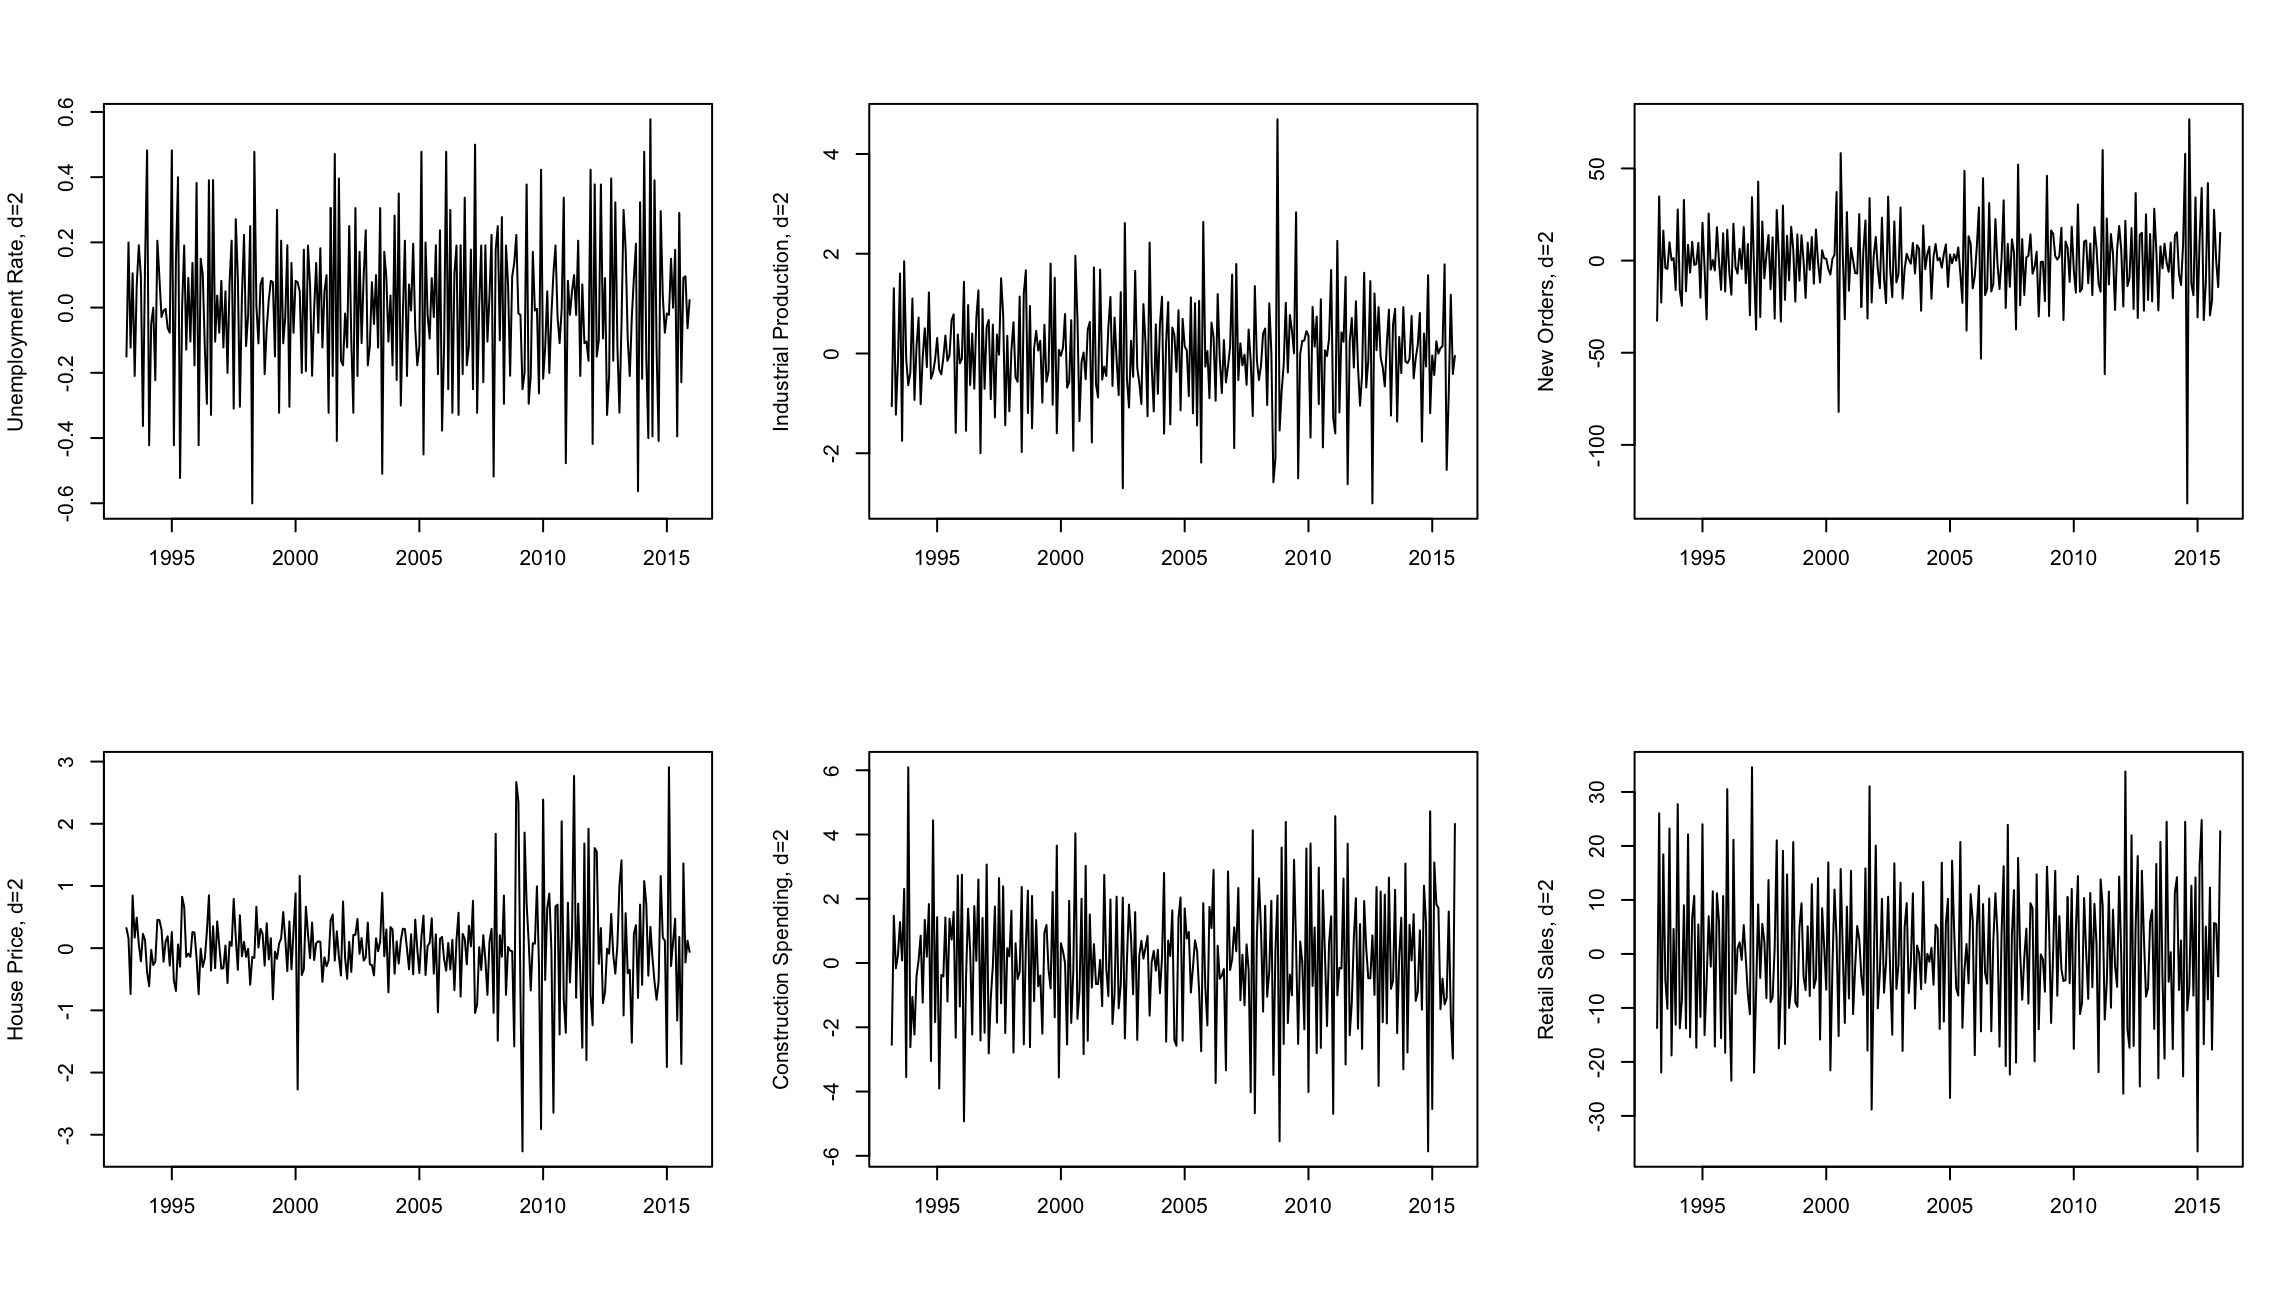
\includegraphics[width=\linewidth]{images/StationaryPred}
  	\end{frame}
 %--------------------------------------------------------------------------------------------------
 
 %-------------------------------------------------------------------------------------------------- 
  	\begin{frame}{ADF Test Results for Predictors, \(d=2\)}
\begin{table}[htb]
		 \centering
		 \begin{tabular}{lllll}
		 \hline
		 \textbf{Variable} & \textbf{Statistic}  & \textbf{p-value}\\ \hline
		  Industrial Production & -9.2333  &\( < 0.01\)\\
		  New Orders &  -8.391  & \( < 0.01\)\\			  
		  House Prices &  -9.104  & \( < 0.01\)\\				  
		  Construction Spending &  -10.447 &  \( < 0.01\)\\
		  Retail Sales &  -10.72 &  \( < 0.01\)\\ \hline
		 \end{tabular}
		 \end{table}
  	\end{frame}
 %--------------------------------------------------------------------------------------------------
 
 %-------------------------------------------------------------------------------------------------- 
  	\begin{frame}{ACF \& PACF Plots}
     	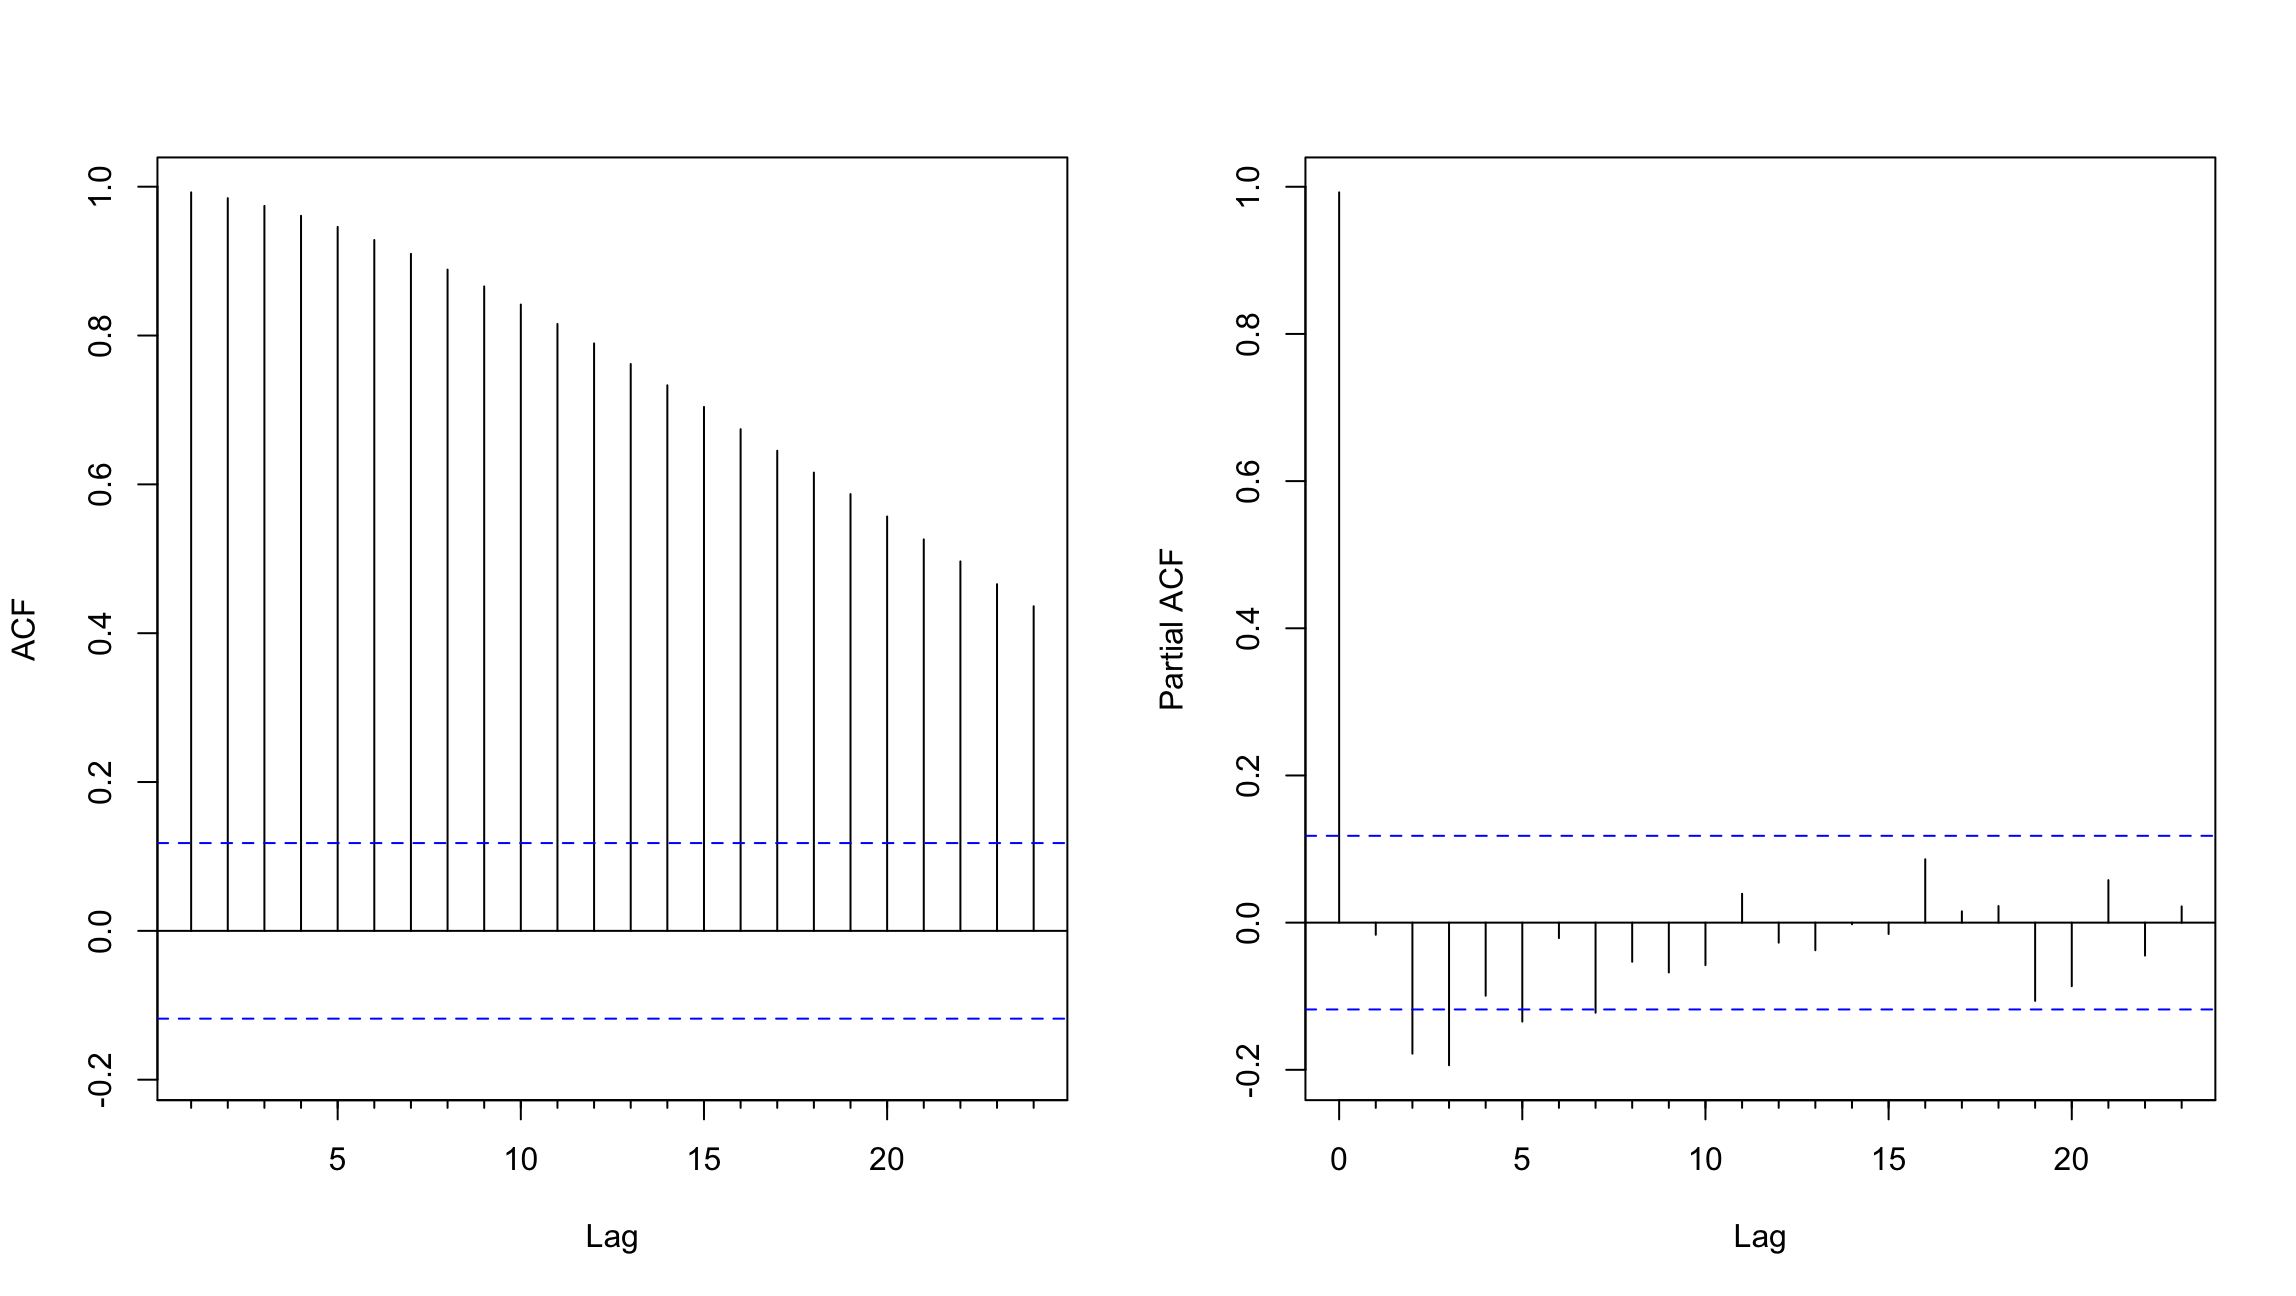
\includegraphics[width=\linewidth]{images/acfpacf}
  	\end{frame}
 %--------------------------------------------------------------------------------------------------
  
  %-------------------------------------------------------------------------------------------------- 
  	\begin{frame}{ACF \& PACF Plots of Second Differences}
     	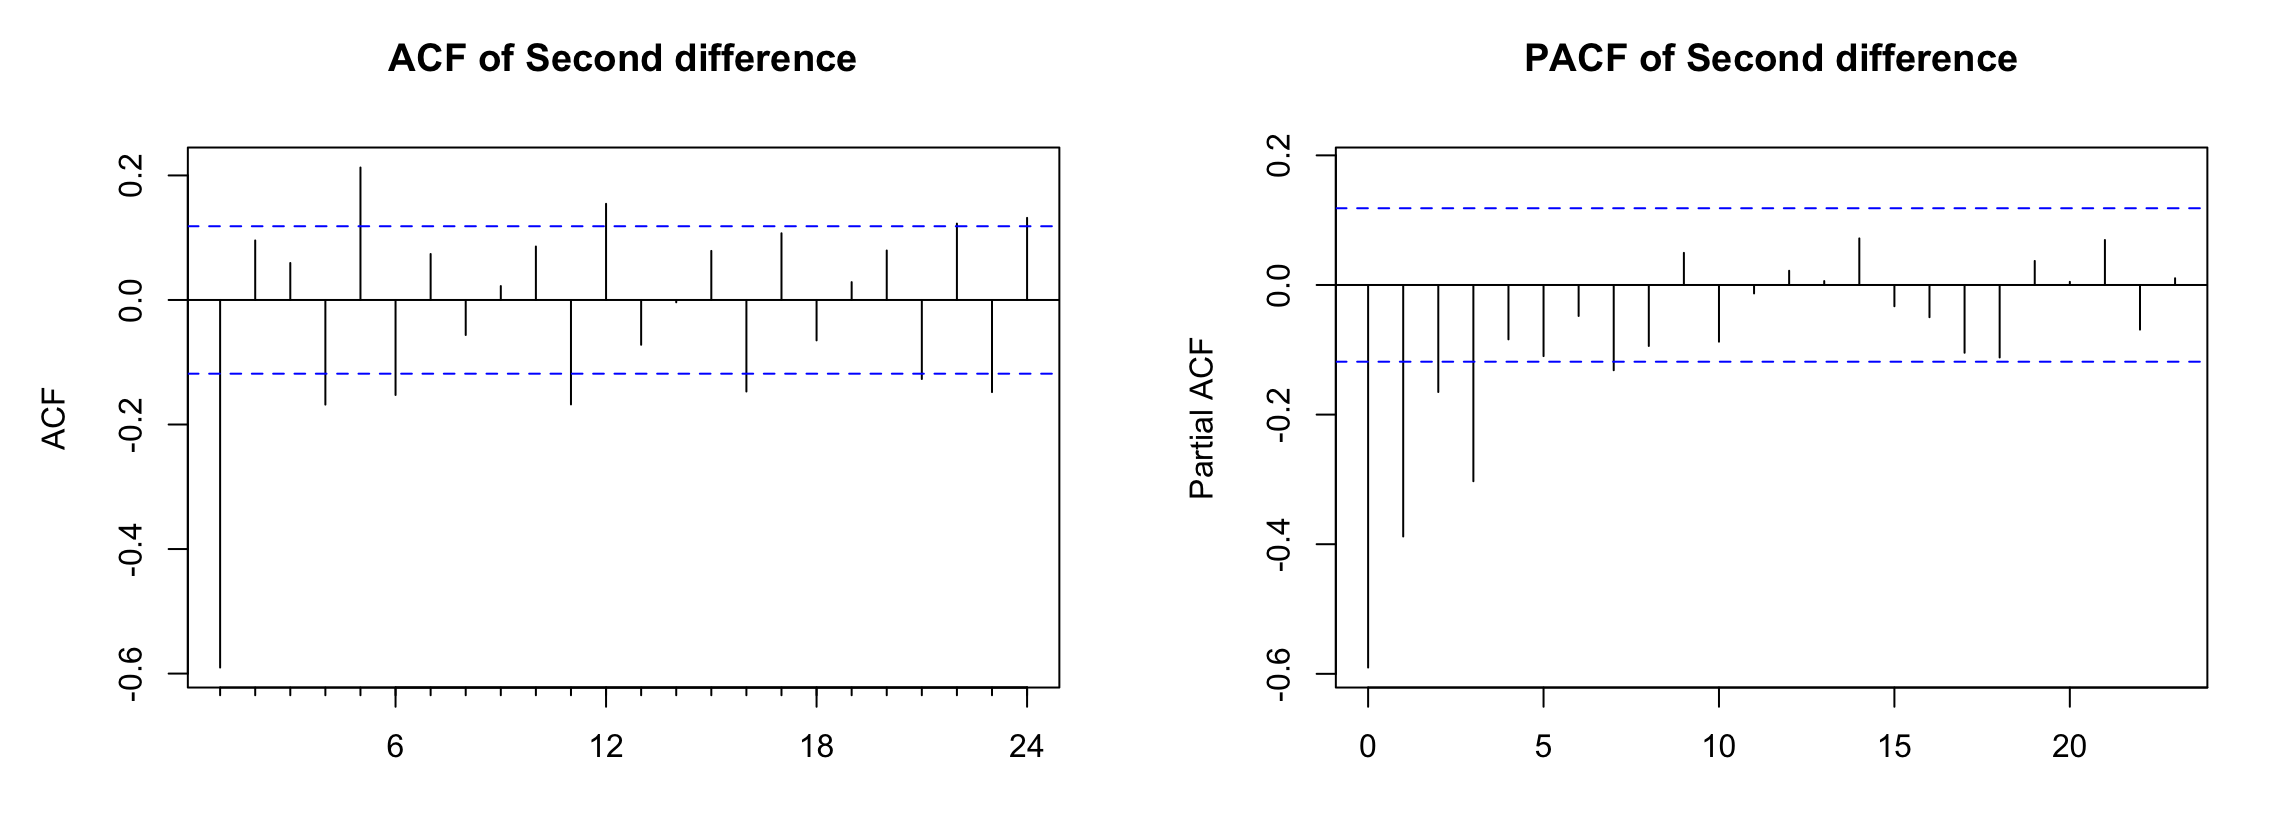
\includegraphics[width=\textwidth]{images/acfpacf2d}
  	\end{frame}
 %--------------------------------------------------------------------------------------------------
  

 \section{Models Considered}
 
 %-------------------------------------------------------------------------------------------------- 
  	\begin{frame}{ARIMA Models Considered}
  		\begin{table}[htb]
\centering
\begin{tabular}{cllrrl}
  \hline
 Model & Order & Reg  & AIC & BIC & Best \\ 
  \hline
1 & 1,2,1 &  NA &   -212.30 & -201.46 & BIC \\ 
  2  & 2,2,2 & NA   & -211.81 & -193.74 &  \\ 
  3  & 3,2,3 &  NA  & -215.48 & -190.19 &  \\ 
  4  & 1,2,1 & X  & -211.56 & -182.65 &  \\ 
  5  & 2,2,2 & X   & -209.83 & -177.32 &  \\ 
  6  & 3,2,3 & X   & -215.10 & -171.74 &  \\ 
  7  & 1,2,1 &  LagX & -222.45 & -193.69 & AIC \\ 
  8  & 2,2,2 &  LagX & -220.70 & -188.35 &  \\ 
  9  & 3,2,3 &  LagX & -217.89 & -174.76 &  \\ 
   \hline
\end{tabular}
\end{table}
  	\end{frame}
 %--------------------------------------------------------------------------------------------------
 
  %-------------------------------------------------------------------------------------------------- 
  	\begin{frame}{VAR Models Considered}
 \begin{table}[htb]
\centering
\begin{tabular}{clllll}
  \hline
 Model & P & Type &  AIC & BIC & Best \\ 
  \hline
1  & 1 & NA  &  -223.67 & -201.97 &  \\ 
  2  & 2 & NA  &   -217.83 & -185.31 &  \\ 
  3  & 1 & Ind  & -256.77 & -231.45 & BIC/AIC \\ 
  4  & 1 & LagX & -216.65 & -195.06 &  \\ 
  5  & 2 & LagX & -212.53 & -180.17 &  \\ 
  6  & 1 & Both  & -245.72 & -220.53 &  \\ 
   \hline
\end{tabular}
\end{table}
  	\end{frame}
 %--------------------------------------------------------------------------------------------------
 
 %-------------------------------------------------------------------------------------------------- 
  	\begin{frame}{Comparison of best ARIMA and VAR models}
\begin{table}[htb]
\begin{tabular}{llll}
  \hline
Model & Type & AIC & BIC \\ 
  \hline
ARIMA \#1 & Univariate ARIMA(1,2,1) &   -212.29 & -201.45  \\ 
ARIMA \#7 & Multivariate ARIMA(1,2,1)  & -222.45 & -193.69   \\ 
VAR \#3 & VAR(1) & -256.76 & -231.45 \\ 
   \hline
\end{tabular}
\end{table}
  	\end{frame}
 %--------------------------------------------------------------------------------------------------
 
 
 \section{Forecast comparisons}
 
 %-------------------------------------------------------------------------------------------------- 
  	\begin{frame}{Multivariate ARIMA(1,2,1)}
  		 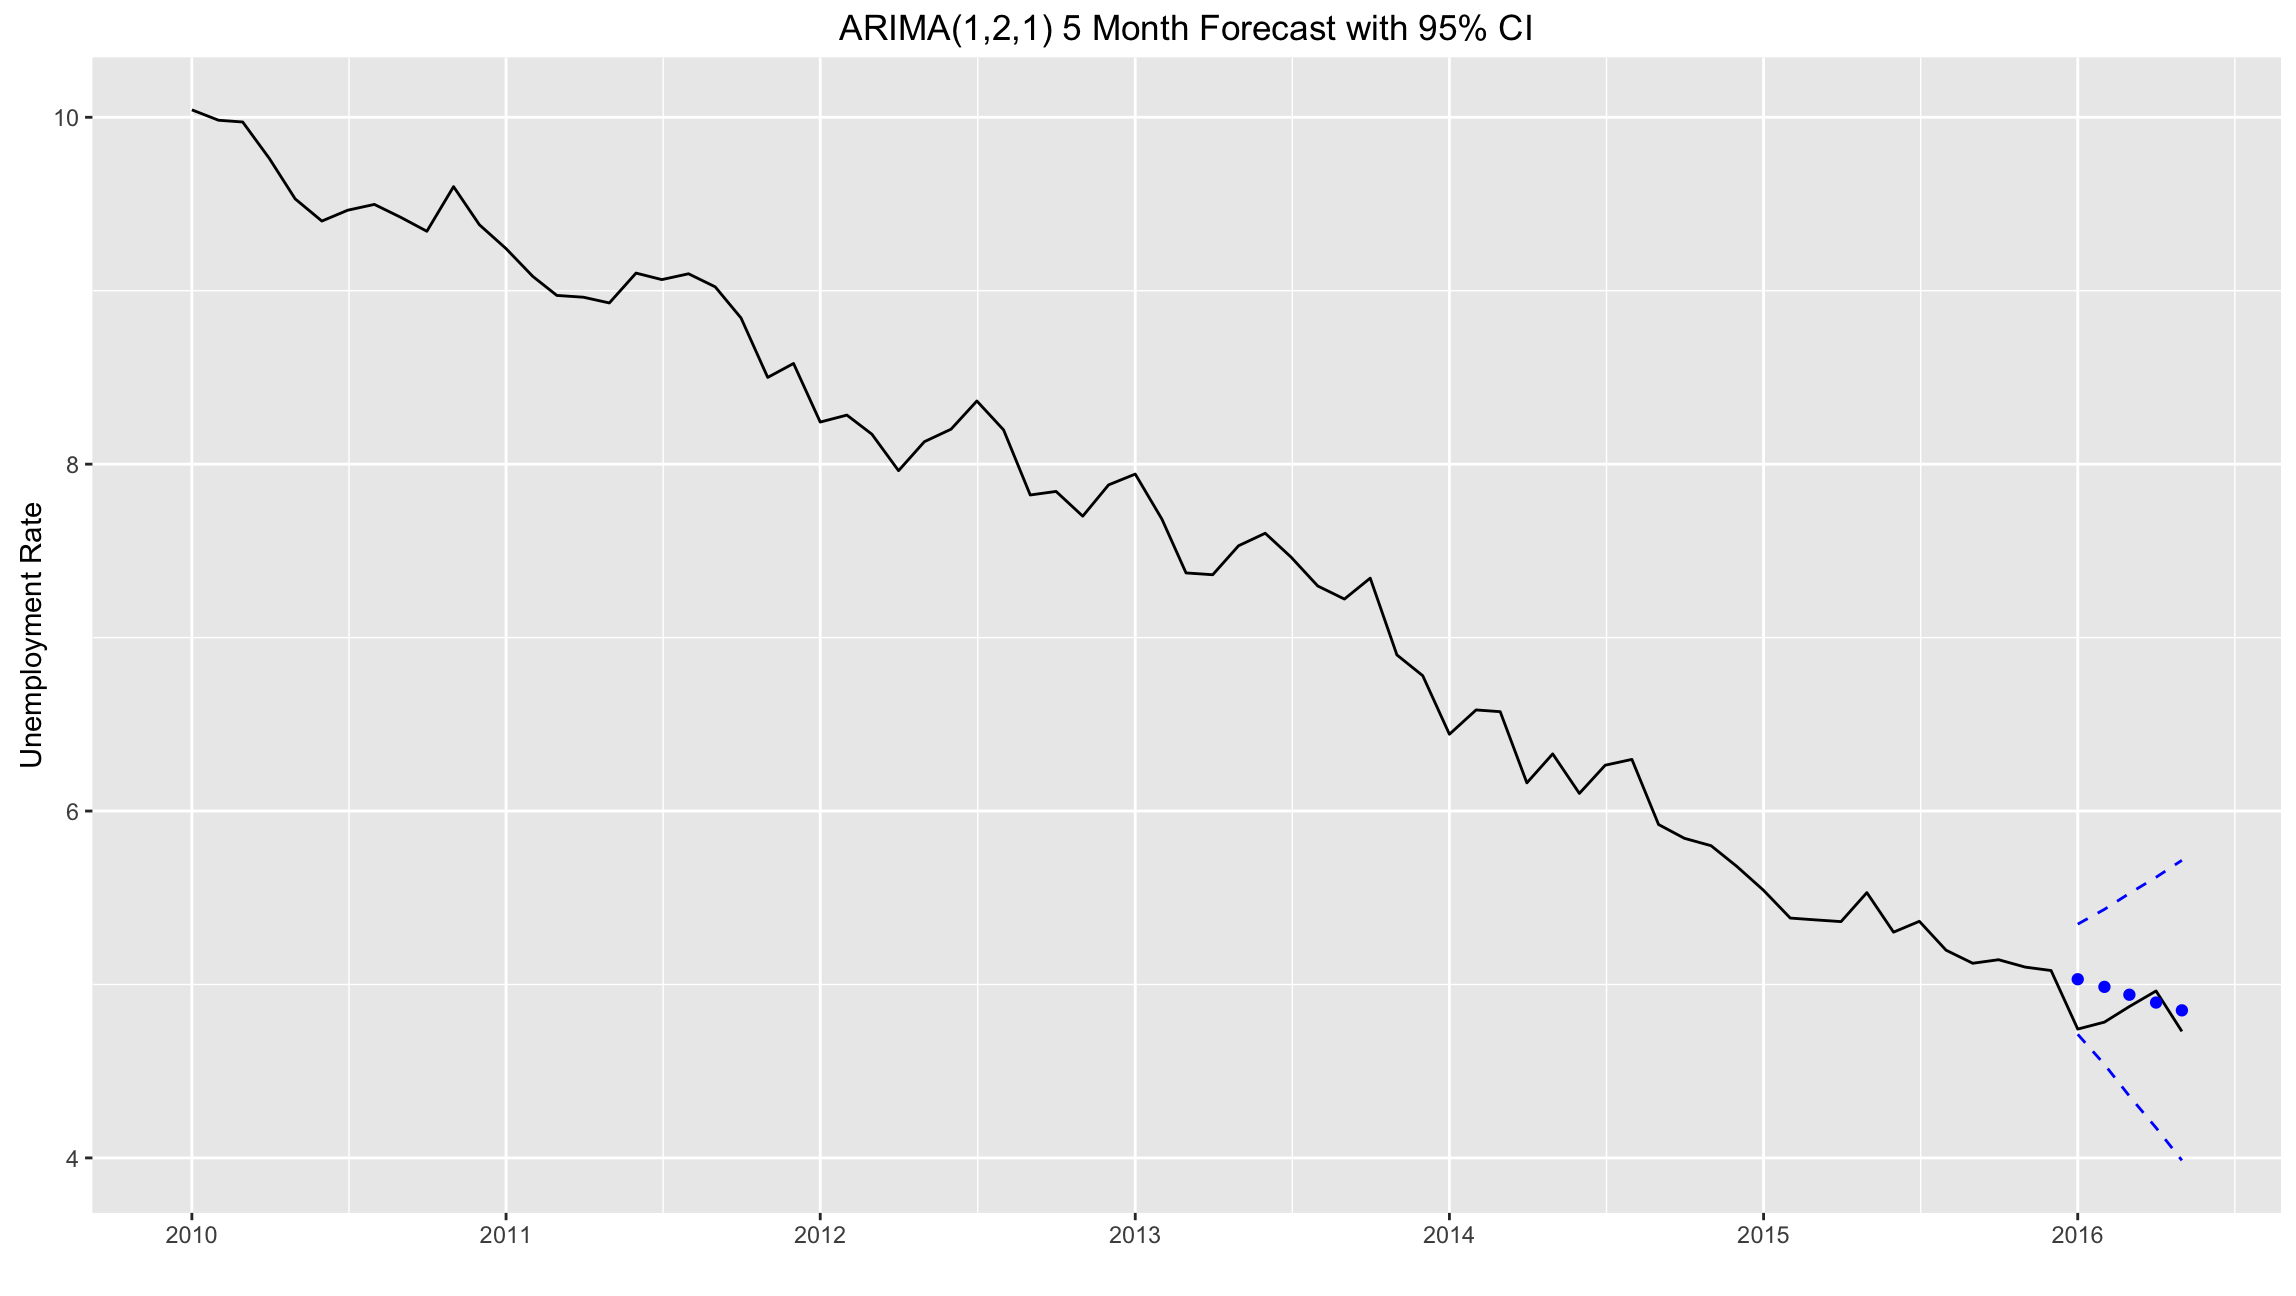
\includegraphics[width=\linewidth]{images/ARIMApred}
  	\end{frame}
 %--------------------------------------------------------------------------------------------------
 
  %-------------------------------------------------------------------------------------------------- 
  	\begin{frame}{VAR(1) }
  		 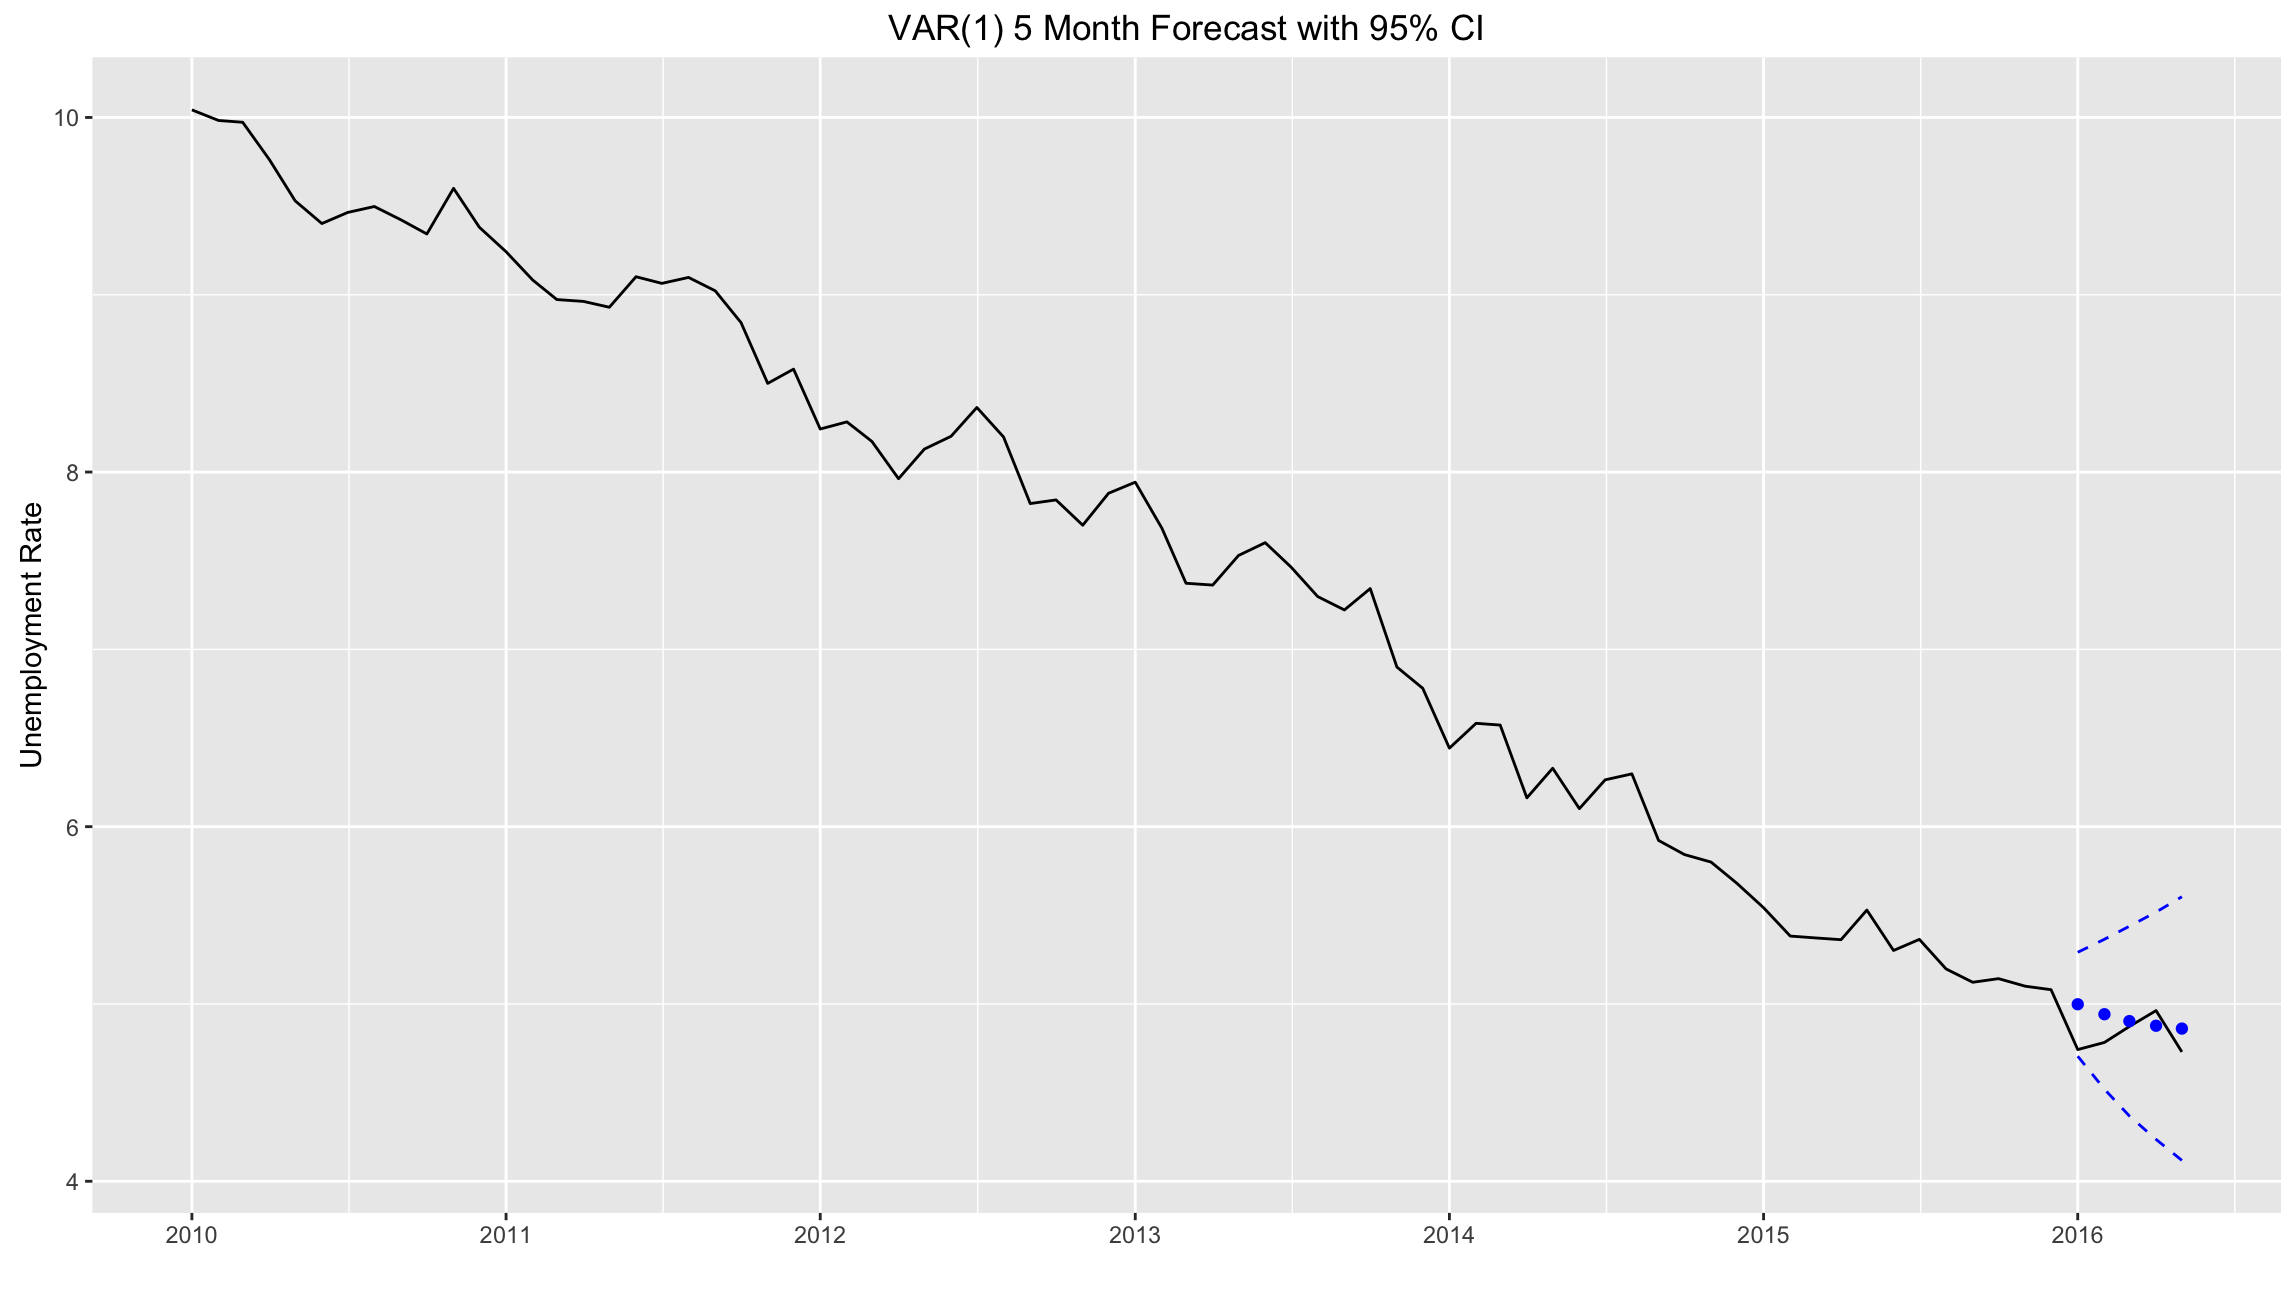
\includegraphics[width=\linewidth]{images/varpred}
  	\end{frame}
 %--------------------------------------------------------------------------------------------------
 
   %-------------------------------------------------------------------------------------------------- 
  	\begin{frame}{Comparison of ARIMA(1,2,1) and VAR(1) }
  		 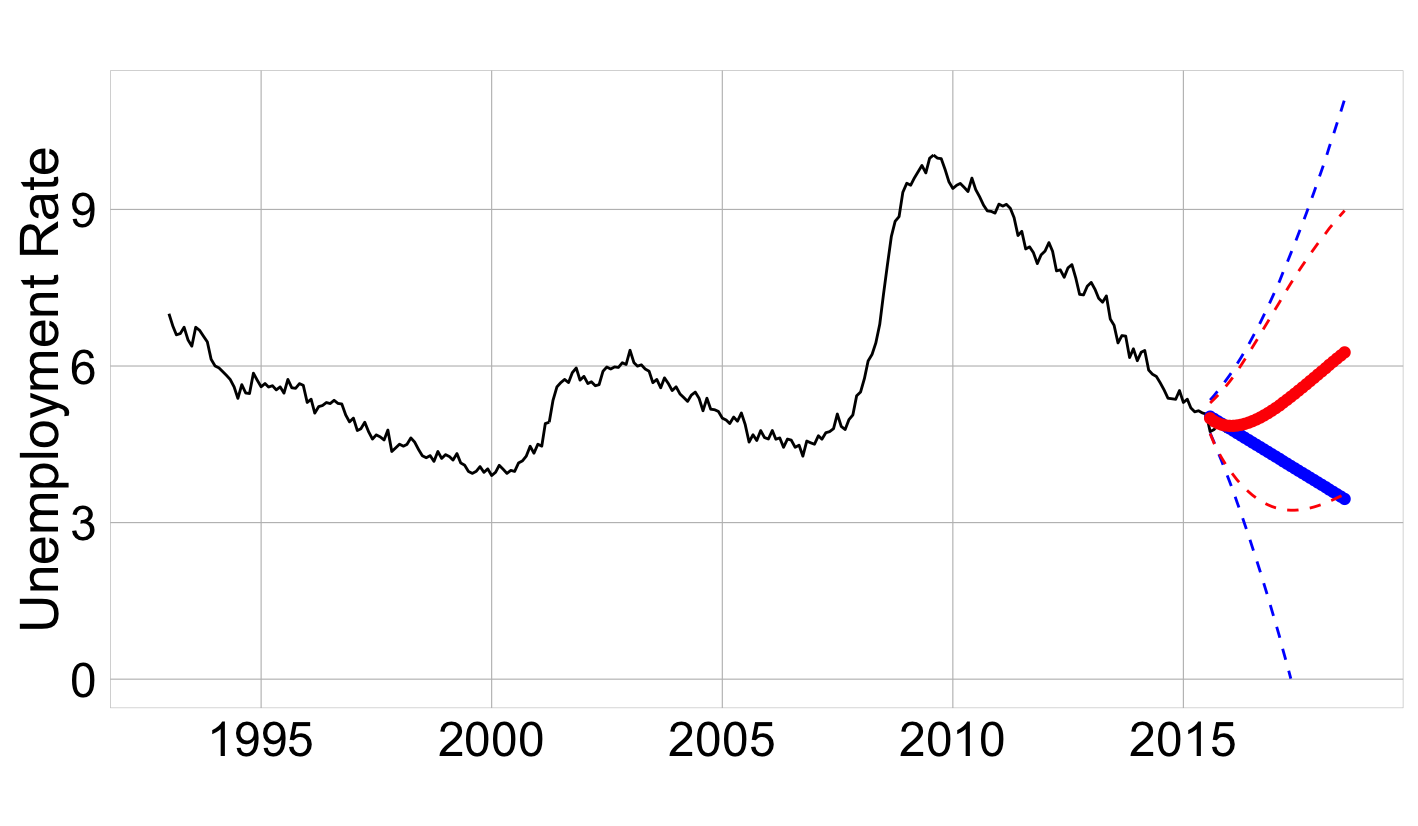
\includegraphics[width=\linewidth]{images/arimavarforecast}
  	\end{frame}
 %-------------------------------------------------------------------------------------------------- 
 
 %-------------------------------------------------------------------------------------------------- 
    \begin{frame}[fragile]{Estimation results for the final model}
\begin{verbnobox}[\small]
-------------------------------------------------------
unem = unem.l1 + constr.l1 + retail.l1 + recession.l1 
		+ const + trend 
-------------------------------------------------------
-------------------------------------------------------
          Estimate Std. Error t value Pr(>|t|)    

unem.l1       0.975191   0.009984  97.677  < 2e-16 ***
constr.l1     0.004262   0.001249   3.412 0.000744 ***
retail.l1    -0.005873   0.001121  -5.241 3.24e-07 ***
recession.l1  0.192394   0.031793   6.051 4.80e-09 ***
const         0.843825   0.201499   4.188 3.82e-05 ***
trend         0.004488   0.000943   4.759 3.17e-06 ***
-------------------------------------------------------
\end{verbnobox}
\end{frame}
 %--------------------------------------------------------------------------------------------------
 
%--------------------------------------------------------------------------------------------------
 
 
  	\begin{frame}{Final Model: VAR(1)}
  		 The final model chose was the VAR(1) with construction spending, retail sales, and the recession indicator as predictors:
  \begin{align*}
  \widehat{\text{U}}\text{nemployment} &= 0.843825_{(0.201499)} +
  0.004488(t)_{(0.000943)}\\ 		
  &+ 0.975191\text{Unemployment}_{t-1 (0.009984)}\\
  &+ 0.004262\text{ConstructionSpend}_{t-1(0.001249)}\\
  &- 0.005873\text{RetailSales}_{t-1(0.001249)}\\
  &+ 0.192394\text{Recession}_{t-1(0.001249)}
  \end{align*}
  	\end{frame}
 %--------------------------------------------------------------------------------------------------



  %-------------------------------------------------------------------------------------------------- 
  	\begin{frame}{Final Model: VAR(1): Predictions}
 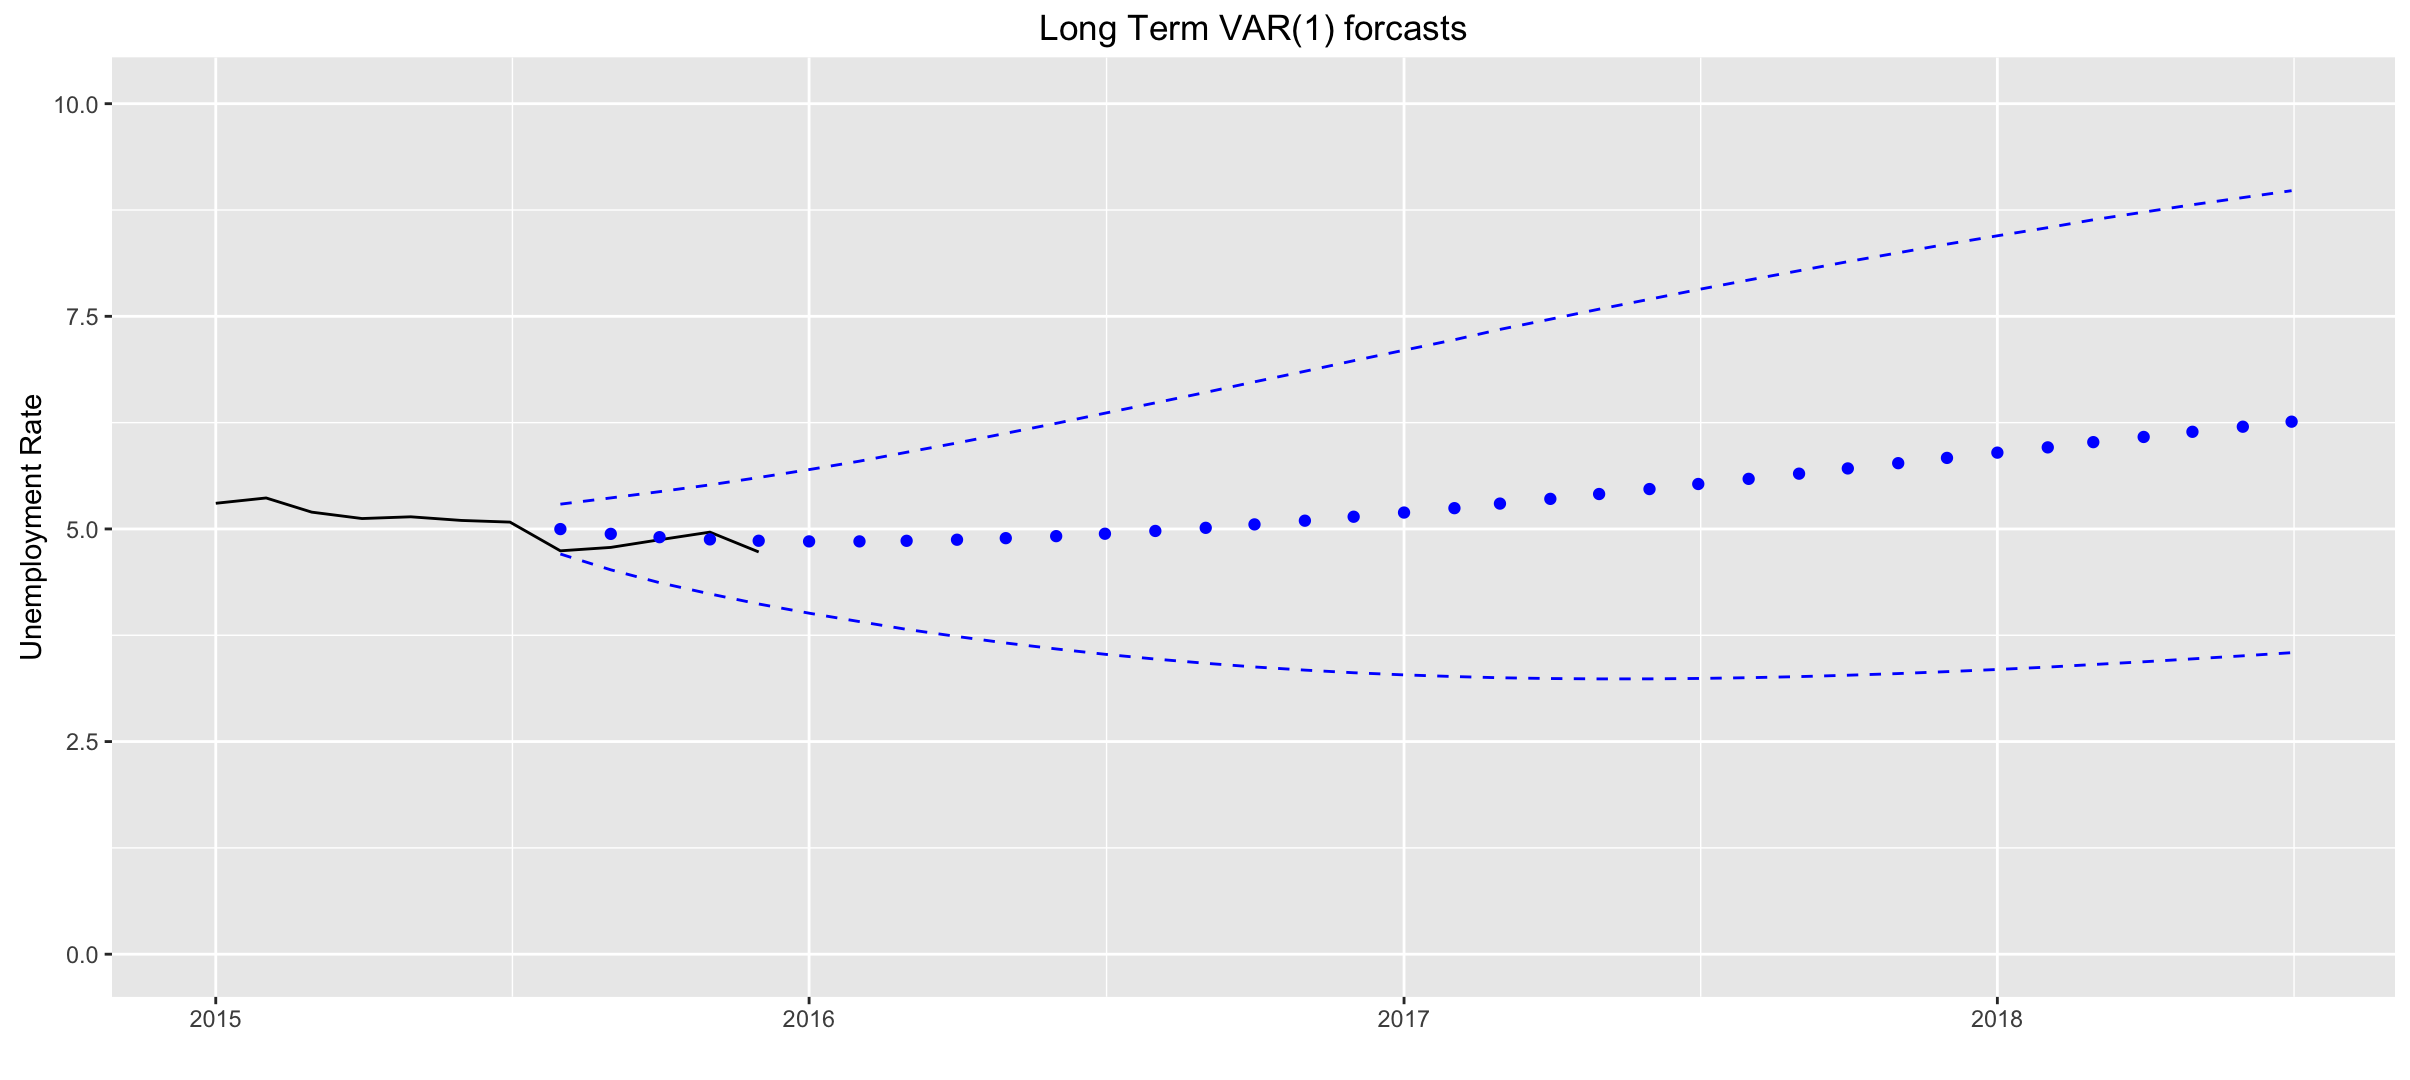
\includegraphics[width=\textwidth]{images/zoomedvar}
  	\end{frame}
 %--------------------------------------------------------------------------------------------------
 
     \end{document}